% Chapter Template

\chapter{Ensayos y resultados} % Main chapter title

\label{Chapter4} % Change X to a consecutive number; for referencing this chapter elsewhere, use \ref{ChapterX}

En este capítulo se detallan los ensayos y mediciones realizados tanto en banco de prueba como en planta para validar los requerimientos planteados. 

%----------------------------------------------------------------------------------------
%	SECTION 1
%----------------------------------------------------------------------------------------

\section{Banco de pruebas}

En la figura \ref{fig:Banco} se puede observar el banco de pruebas utilizado. El osciloscopio es el modelo Hantek DSO2D10 \citep{web_hantek} y la fuente regulable es una YIHUA 305D \citep{web_yihua}. En la PC se ejecuta un programa de monitor serial llamado PuTTy \citep{web_putty} que se emplea para visualizar de forma simplificada el mensaje que el sistema envía a la red CAN.

\begin{figure}[htbp]
	\centering
	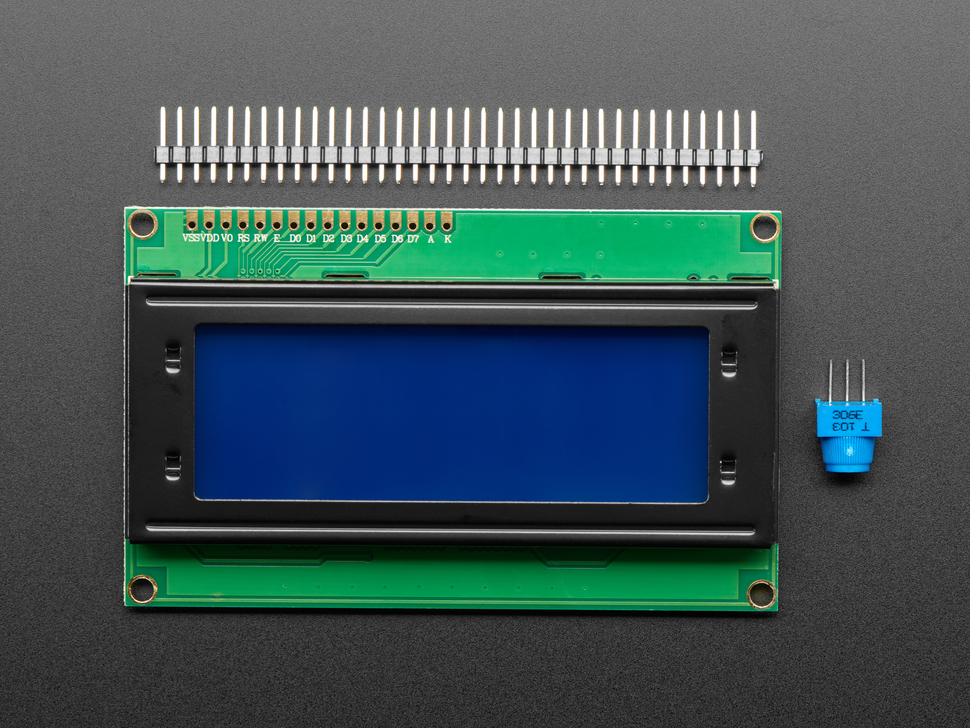
\includegraphics[scale=1]{./Figures/LCD.jpg}
	\caption{Banco de pruebas utilizado para verificaciones - ARAMR FIGURA}
	\label{fig:Banco}
\end{figure}


\section{Ensayo de mensajes CAN}

En la figura \ref{fig:niv_señal} se puede ver una de trama CAN medida con el osciloscopio. Se identifican las señales CAN-H y CAN-L con valores de tensión acordes a lo esperado. Es importante notar la ausencia de ruido en la señal, que indica la correcta slección de los resistores de terminación.

\begin{figure}[htbp]
	\centering
	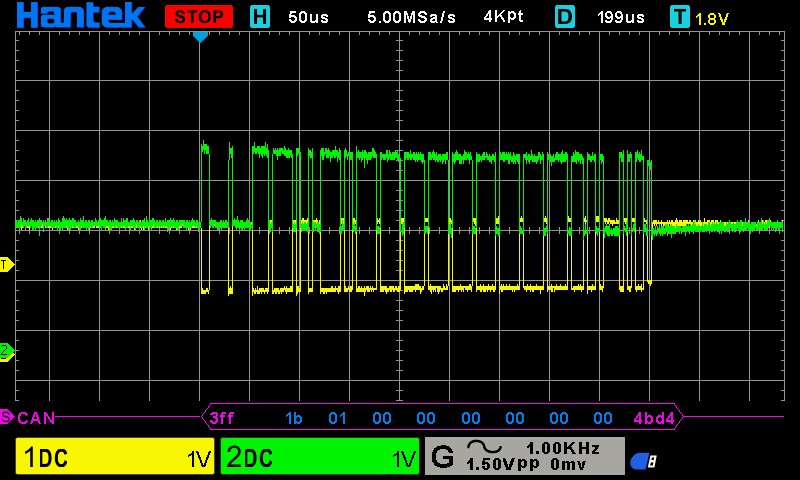
\includegraphics[scale=0.6]{./Figures/Message_Change_Operation_Mode_CONFIG.jpg}
	\caption{Niveles de señal CAN en osciloscopio}
	\label{fig:niv_señal}
\end{figure}

En la figura \ref{fig:tiempo_bit_can} se presenta la medición de tiempo tomada desde el osciloscopio para uno de los bits de un mensaje CAN. Se puede ver en la esquina superior izquierda el valor de tiempo obtenido de 4.1 $\mu$s, que es lo esperado según lo explicado en la sección \ref{comunicacion_can}. Este tiempo implica una velocidad de transmisión de 250 kb/s.

\begin{figure}[htbp]
	\centering
	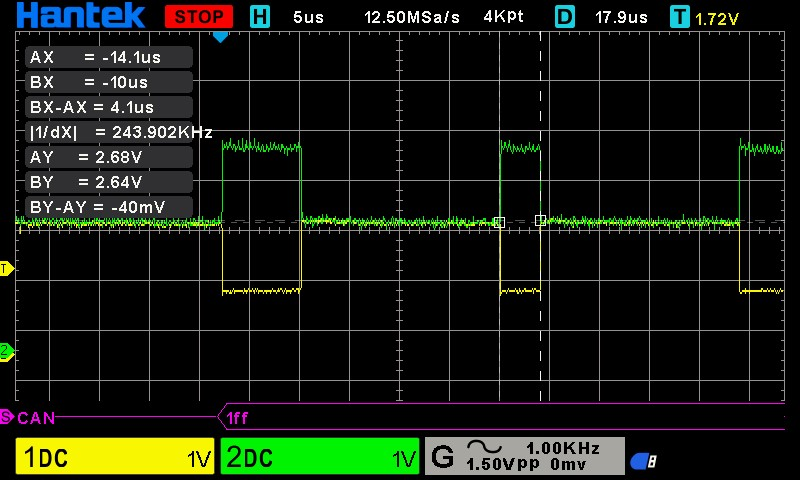
\includegraphics[scale=0.6]{./Figures/bit_time_can.jpeg}
	\caption{Medición de tiempo de bit}
	\label{fig:tiempo_bit_can}
\end{figure}

Los mensajes de la tabla \ref{tab:tipos_mensajes_CAN} fueron probados uno a uno, tanto el identificador como el payload correspondiente. Se verificó que los sistemas SN-17 conectados realicen las acciones correctas.

Como ejemplo, la figura \ref{fig:mot_calib} presenta una imagen tomada del osciloscopio para la instrucción de calibrar motor (código: 0x0c). En la parte inferior puede observarse el decodificador CAN que el osciloscopio trae incorporado que marca correctamente la instrucción. También se percibe el identificador del mensaje (código: 0x0b) compuesto por el identificador del motor (0x05) y el bit final que indica que es un mensaje desde el dispositivo controlador. El resto de los bytes de data se marcan en 0 ya que no es necesario envíar más información para este tipo de mensaje. Los últimos bytes pertenecen al CRC.

\begin{figure}[htbp]
	\centering
	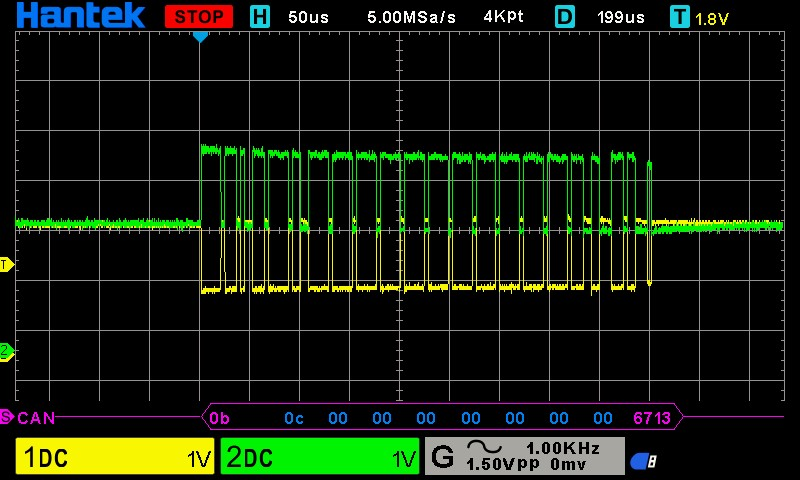
\includegraphics[scale=0.6]{./Figures/Motor_Calibrate.jpg}
	\caption{Instrucción calibrar motor}
	\label{fig:mot_calib}
\end{figure}

Otro ejemplo de mensaje puede visualizarse en la figura \ref{fig:mot_move} en la que se envía al motor un comando manual de movimiento angular (código: 0x10), en dirección en contra de las agujas del reloj (código 0x01), un ángulo de 360 grados (códigos: 0x01 y 0x68). En este caso, como el ángulo es un número que requiere más de un byte para su representación aparece descompuesto en el mensaje. Al recibir el mensaje, el motor realiza el giro estipulado.

\begin{figure}[htbp]
	\centering
	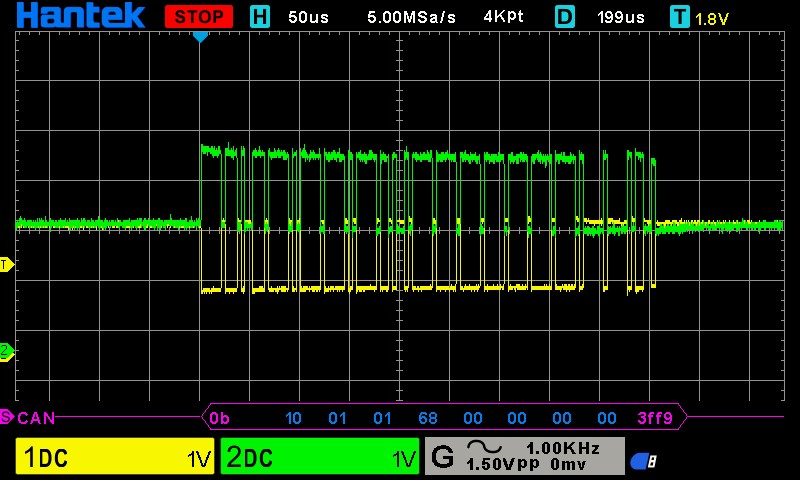
\includegraphics[scale=0.6]{./Figures/Motor_Manual_Move_CCW_360DEG.jpg}
	\caption{Instrucción manual mover motor}
	\label{fig:mot_move}
\end{figure}


\section{Ensayos eléctricos}

Los ensayos eléctricos se realizaron sobre la plaqueta de control conectada directamente a la fuente de alimentación regulable configurada a 24 V y sin ningún otro dispositivo conectado. Se hicieron mediciones utilizando un multímetro para verificar que los niveles de tensión del sistema fueran los apropiados. Las verificaciones realizadas se presentan en la Tabla \ref{tab:verificaciones_electricas}.

\begin{table}[h]
	\centering
	\caption[Verificaciones eléctricas]{Verificaciones eléctricas}
	\begin{tabular}{c c c}    
		\toprule
		\textbf{Ensayo} 	 & 		\textbf{Descripción} \\
		\midrule
		Regulador & 5 V a la salida del regulador\\
		Referencias fuente & 24 V en bornes de referencia de fuente \\
		Referencias regulador & 5 V en bornes de referencia de controlador \\
		IOs controlador & 5 V en bornes de IOs de controlador \\		
		IOs puenteadas 	& 24 V en IOs aisladas puenteadas a tensión de entrada \\
		IOs	diferidas	& IOs aisladas a 12 V con alimentación de sistema a 24 V \\
		\bottomrule
		\hline
	\end{tabular}
	\label{tab:verificaciones_electricas}
\end{table} 

Las salidas PNP del sistema se ensayaron con una conexión a un PLC Omron NX102 \citep{web_nx102}. Las cuatro se conectaron a un módulo de entradas DC NX-ID5442. Se comprobó que al activar las salidas el PLC las recibe de forma correcta.

Con las entradas del sistema se realizó un procedimiento similar, conectando cada una a un módulo de salidas PNP NX-OD5256. Se activaron las salidas desde el PLC y se verificó que se recibe la señal desde el sistema.

VER DE AGREGAR UNA IMAGEN CON EL DISPOSITIVO CONECTADO AL PLC

\section{Ensayos de mensajes UART-USB}

En la medición de la comunicación con la PC se utilizó el mismo banco de medición conectando la punta del osciloscopio al bus de datos UART-USB.

En la figura \ref{fig:signal_uart} se muestra una imagen del osciloscopio con las mediciones realizadas sobre la señal de UART. Se verifica el tiempo de bit correcto de 106 $\mu$s, correspondiente a un \textit{baudrate} de 9600 y el nível de tensión de 5 V. Se comprobó que los mensajes enviados y recibidos fueran correctos y que el sistema actuara acorde a lo esperado.

\begin{figure}[htbp]
	\centering
	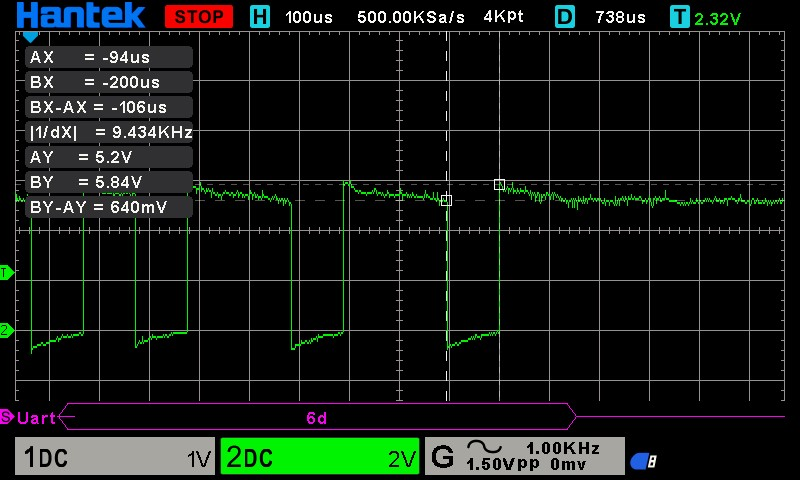
\includegraphics[scale=0.6]{./Figures/bit_time_uart.jpeg}
	\caption{Medición de señal UART}
	\label{fig:signal_uart}
\end{figure}

Por otro lado, se verificó que los niveles de señal USB, obtenida luego del integrado CY7C64225 fueran correctos. En la figura \ref{fig:signal_usb} se presenta la medición obtenida, donde se ve la señal diferencial correspondiente al protocolo USB en modo \textit{full-speed}. Se puede comprobar el nivel de tensión de 3 V y el tiempo de bit de 83 ns. Esto corresponde con la especificación del dispositivo.

\begin{figure}[htbp]
	\centering
	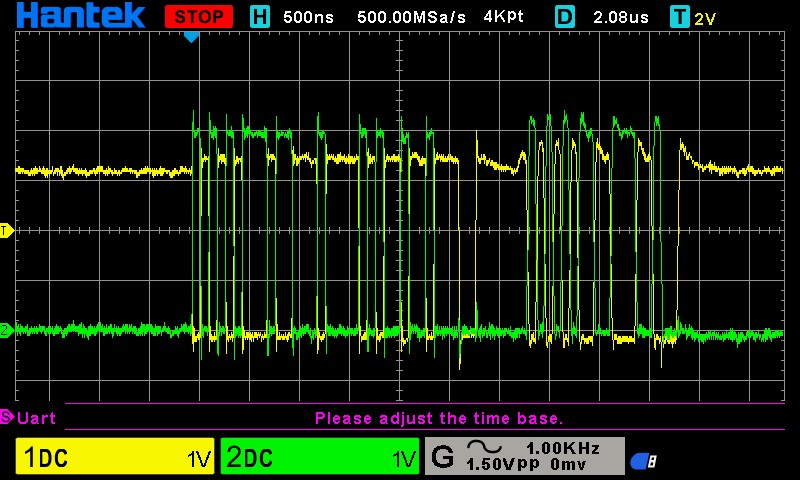
\includegraphics[scale=0.6]{./Figures/msg_usb.jpeg}
	\caption{Medición de señal USB}
	\label{fig:signal_usb}
\end{figure}

\section{Pruebas de funcionamiento en planta}

El dispositivo fue ensayado en la planta de Cambre ICyFSA donde se conectó en una línea de ensamble automática en desarrollo. Esta línea cuenta con varios sistemas SN-17 montados para realizar distintas actuaciones mecánicas. También, la línea cuenta con un PLC Omron NX-102 que controla el proceso. La figura \ref{fig:esquema_conexion_planta} muestra el esquema de conexionado empleado para realizar las pruebas del sistema en la línea de ensamblaje.

\begin{figure}[htbp]
	\centering
	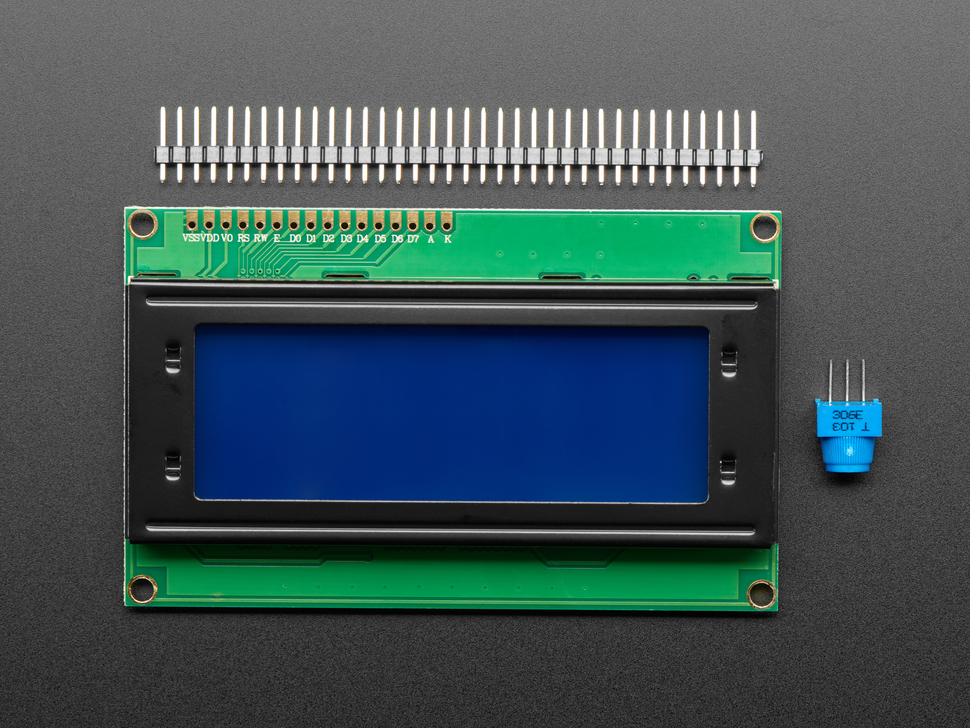
\includegraphics[scale=1]{./Figures/LCD.jpg}
	\caption{Esquema de conexionado en planta - ARAMR FIGURA}
	\label{fig:esquema_conexion_planta}
\end{figure}

Con la disposición explicada se realizó la programación de los sistemas SN-17 de la línea y se monitoreó su operación. Se comprobó que el sistema muestre correctamente el estado de funcionamiento en operación de los SN-17 y el número de programa e instrucción en ejecución de cada uno de ellos. En la figura \ref{fig:pantalla_monitoreo} se observa la información de monitoreo que ofrece el SCI-CAN en el display de los motores conectados en operación. El primer número indica el número de programa en ejecución por el motor, el segundo el número de instrucción de ese programa.

\begin{figure}[htbp]
	\centering
	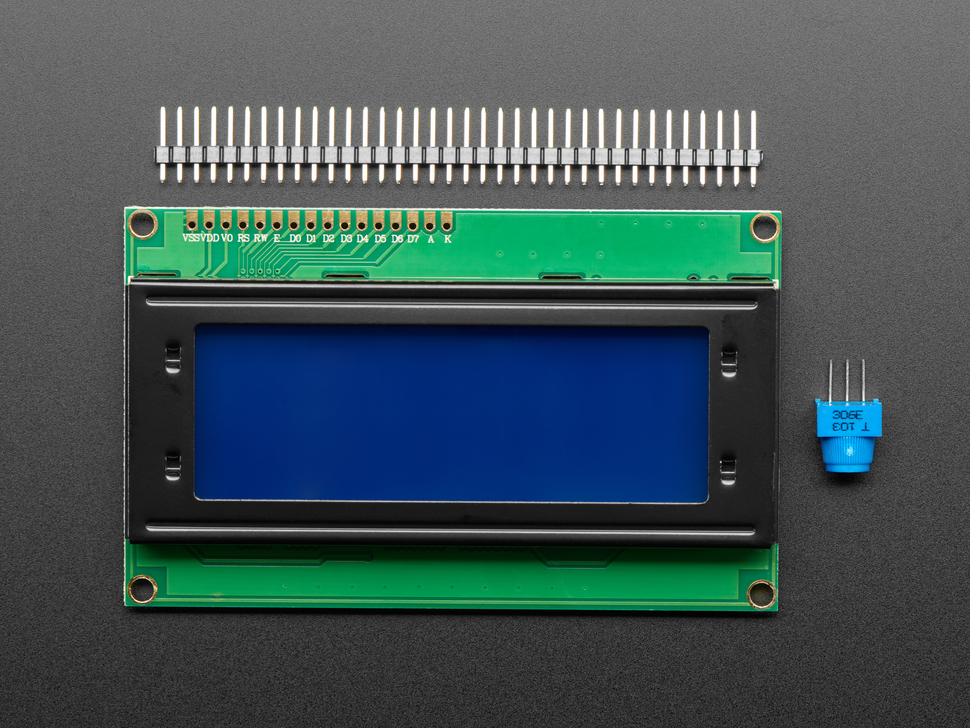
\includegraphics[scale=1]{./Figures/LCD.jpg}
	\caption{Monitoreo de SN-17 - ARAMR FIGURA INCLUIR ERROR}
	\label{fig:pantalla_monitoreo}
\end{figure}

También, se verificó la comunicación a través de señales discretas con el PLC. Como se puede observar en el display del sistema de la figura \ref{fig:pantalla_monitoreo}, en caso de que un sistema SN-17 se encuentre en error se visualiza junto al número de instrucción. En estos casos, el sistema envía una señal al PLC para indicarle el estado de error.

En la figura \ref{fig:sistema_en_planta} se muestra el dispositivo montado en la línea de ensamblaje automático en Cambre ICyFSA.

\begin{figure}[htbp]
	\centering
	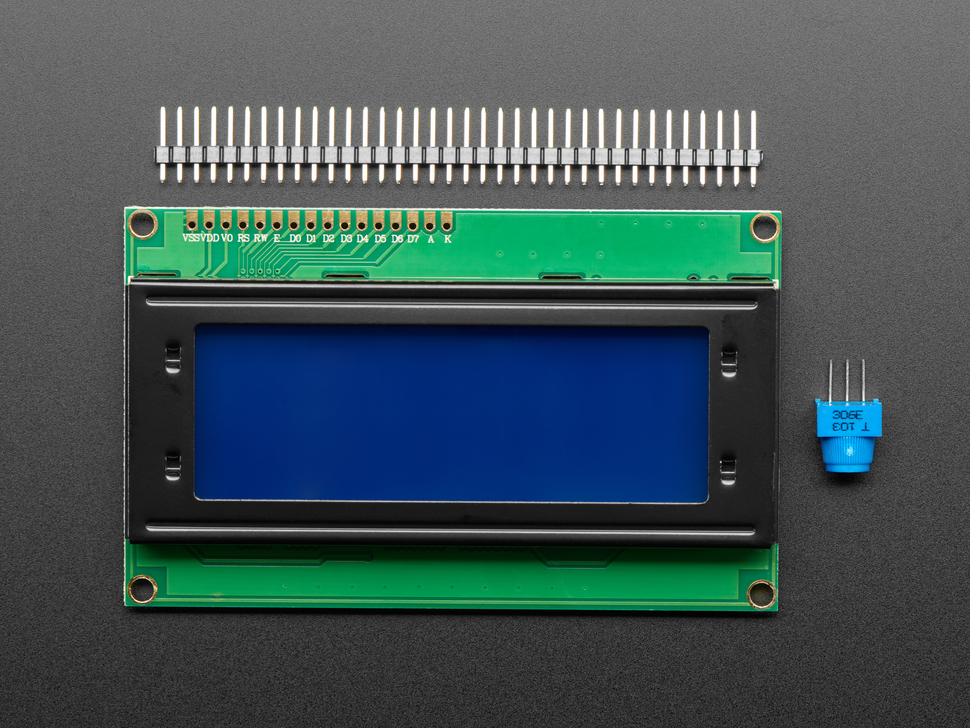
\includegraphics[scale=1]{./Figures/LCD.jpg}
	\caption{Sistema montado en línea de ensamble automático - ARAMR FIGURA}
	\label{fig:sistema_en_planta}
\end{figure}

\section{Comparación con estado del arte}

